%%%%%%%%%%%%%%%%%%%%%%%%%%%%%%%%%%%%%%%%%%%%%%%%%%%%%%%%%%%%%%%%%%%%%%%%%%%%%%%%%
%%%%%                                RESULTS                                 %%%%
%%%%%%%%%%%%%%%%%%%%%%%%%%%%%%%%%%%%%%%%%%%%%%%%%%%%%%%%%%%%%%%%%%%%%%%%%%%%%%%%%

In this section we present our main results. Initially, we use the \textit{static} model
to estimate an elasticity of the MW to rents of about 0.026 (s.e. 0.013). We check the
robustness of our results by progressively including plausible controls for the dynamics 
of the local economy, and by including parametric local trends. Our results do not change.

Following the reasoning in \autoref{sec:empirical_strategy}, we then present estimates of 
\textit{dynamic} models. Results show a short-lived dynamic effect, mainly over the two
months following the policy: we estimate the cumulative impact of a 10 percent MW increase 
to be between 0.5 and 0.6 percent over the course of the 5 months after the policy change. 
We find no pre-trends in our estimations, which under the assumption of fixed housing supply 
we interpret as evidence in favor of our identification assumption. We indirectly assess the 
validity of the housing supply assumption by running a placebo regression where we replace 
our main dependent variable with the number of listings \textit{for sale} in Zillow. 
Finally,we estimate panel models that include the lagged dependent variable as control in 
the appendix.

% SH: I removed the below. I don't think we need into that much detail in this overview

%, where we don't find any significant effect.\footnote{This exercises implicitly assumes 
%the presence of of a correlation between the number of listings \textit{for rent} and 
%\textit{for sale} on Zillow.}


% SH: I removed references to particular subsections. I'm happy to include those, but we have to be
% consistent. If we decide to do that we should reference all subsections.

% SH: Following Jesse's comments, I removed the comment on how our main estimate can be seen as 
% a lower bound from the paragraph below

We conduct two exercises to assess to what extent our results estimated in the Zillow sample 
are representative of the underlying average treatment effect across the population of urban
zipcodes. First, we re-estimate our static model via weighted regression, where weights for 
each zipcode are constructed so that our sample matches demographic statistics of the top 100 
CBSA.  As expected, we find that the estimated elasticity increases slightly. Second, we 
re-estimate our static model on a expanded sample that includes the whole set of zipcodes 
available in the Zillow data, no matter the data they ``entered'' the panel. We account for 
changes in zipcode composition by controlling for \textit{entry cohort} $\times$ \textit{time} 
fixed effects. Our results show robust to this exercise.

% SH: I removed references to experienced MW below, which will go in the experienced_MW section
%     I also removed discussion of the benchmarking

After establishing the robustness of our results, we follow the strategy outlined in 
\autoref{sec:strategy_heterogeneity} to investigate how the incidence of the effect may vary 
across the distribution of zipcode characteristics. First, we use LODES data to proxy for MW 
workers residence and workplace location to show how effects disproportionately affect those 
zipcode that are more likely to have low-wage workers as residents. Secondly, we estimate the 
heterogeneous impact of MW changes across the distribution of several census-based 
demographics. The results indicate that the effects are concentrated in poorer, less-educated, 
and more African-American zipcodes. 

Importantly, all regressions cluster standard errors at the state level so to match the main 
source of variation of MW changes.

%%%%%%%%%%%%%%%%%%%%%%%%%%%%%%%%%%%%%%%%%%%%%%%%%%%%%%%%%%%%%%%%%%%%%%%%%%%%%%%%%
\subsection{Baseline Results}\label{sec:baseline_results}

\autoref{tab:did_main} presents results from the static model defined in \autoref{eq:did}. In 
column 1, we show the classic two-way fixed effects --zipcode and monthly date-- estimated in 
first differences. A potential threat to the identification is the presence of unobserved shocks 
systematically affecting MW and rent changes. In order to account for this possibility, in 
columns 2 to 5 we show results of several models with different sets of controls that proxy for 
shocks to the local economy in columns 2, 3, and 4. As we discussed in the previous section, 
the controls are taken from the QCEW and thus vary either at the county-month or county-quarter 
level. While this prevents us from studying the presence of time-varying confounding factors at 
the zipcode-level, the controls plausibly capture shocks correlated with MW changes, which are 
also decided at higher levels of aggregation than the zipcode --i.e., city, county, or state 
levels. In fact, if there are underlying factors affecting MW changes that also affect 
zipcode-level rents, they would likely arise from this larger geographic units. 

Wages, employment and the number of establishments are also potentially affected by MW changes,
which may result in an invalid regression due to the use of ``bad controls'' 
\parencite{AngristPischke2009}. To avoid this problem we only include controls from industries 
that are unlikely to be affected by MW policies. These are ``Professional and Business Services", 
%% UPDATE SECTORS AFTER REVIEW
``Information", and ``Financial activities". The controls used in the regression are as follows:
column 2 includes average weekly wages at the county-quarter level; column 3 controls for 
employment at the county-month level; column 4 uses the number of establishments in the 
corresponding county and quarter. We include the difference in the log of each variable in our
regressions. Finally, in column 5 we jointly account for all sets of controls. All specifications 
return very similar results. A 10 percent increase in the MW leads to a 0.26 percent increase 
in rents. 

One may still worry that heterogeneous dynamics in local markets at the zipcode level bias our 
results. To account for that, \autoref{tab:did_trend} in the appendix reports estimation 
results of the static model that include zipcode-specific linear and quadratric trends as controls. 
Reassuringly, the coefficient of interest does not change.

\begin{table}[h!]
    \caption{The static effect of MW increases on rents}
    \label{tab:did_main}
    \centering
    {
\def\sym#1{\ifmmode^{#1}\else\(^{#1}\)\fi}
\begin{tabular}{l*{3}{c}}
\hline\hline
          &\multicolumn{1}{c}{(1)}&\multicolumn{1}{c}{(2)}&\multicolumn{1}{c}{(3)}\\
          &\multicolumn{1}{c}{D.ln\_med\_rent\_psqft}&\multicolumn{1}{c}{D.ln\_med\_rent\_psqft}&\multicolumn{1}{c}{D.ln\_med\_rent\_psqft}\\
\hline
D.ln\_mw   &   0.0260\sym{**} &   0.0257\sym{**} &   0.0255\sym{**} \\
          & (0.0128)         & (0.0120)         & (0.0117)         \\
\hline
Zipcode-specifc linear trend&       No         &      Yes         &      Yes         \\
Zipcode-specific linear and square trend&       No         &       No         &      Yes         \\
R-squared &    0.022         &    0.024         &    0.026         \\
Observations&   112232         &   112232         &   112232         \\
\hline\hline
\end{tabular}
}

    \begin{minipage}{0.9\textwidth} \footnotesize
		% UPDATE NOTES
		\vspace{3mm} 
		\textit{Notes}: The table reports coefficients from versions of \autoref{eq:did} 
		estimated on the balanced panel of zipcode-months described in \autoref{sec:data}. 
		The dependent variable is the difference in the natural logarithm of median	rents 
		per square foot in the Single Family, Condos and Condominiums category in Zillow, 
		whereas the main independent variable is the difference in the natural logarithm of 
		the statutory minimum wage. All columns control for monthly date fixed effects. In 
		addition, columns (2) to (5) include economic controls from the industries 
		%%% UPDATE SECTORS AFTER REVIEW
		``Professional and business services'', ``Information'', and ``Financial activities'' 
		from the QCEW. Wage controls are the difference in the natural logarithm of average 
		weekly wages, employment controls are the difference in the natural logarithm of 
		employment, and establishment count controls refer to the difference in the natural 
		logarithm of number of establishments. Wages and establishment count vary at the 
		county-quarter level, whereas employment varies at the county-month level. Standard 
		errors are clustered at the state level. Significance codes: *** $p < 0.01$, ** 
		$p < 0.05$, * $p < 0.1$.
	\end{minipage}
\end{table}

A causal interpretation of the estimates from the static model rely on a \textit{strict exogeneity} 
assumption, which states that minimum wage changes are orthogonal to past and future changes in rents.
This assumption may not hold in practice. One way to assess its validity is by a classical 
``pre-trends test''. To conduct that test we estimate a dynamic model with leads and lags of MW 
changes, and evaluate whether coefficients on leads are zero. Under the assumption that the MW does 
not affect the supply of rentals, economic shocks leading to both increases in minimum wages and 
rents would show up as non-zero pre-trends. A second problem with the strict exogeneity assumption, 
although a less concerning one, is that it presupposes no dynamic effect of MW changes. This 
restriction is eased by the inclusion of lags in the model.

In \autoref{fig:fd_models_main}, we plot the estimated coefficients of the \textit{dynamic} model 
(including the full set of economic controls) together with 90 \% confidence intervals. In the appendix 
(\autoref{tab:dynamic_lags_leads_main}) we show the full set of coefficients, fit statistics, and a 
p-value of an F-test of the hypothesis that all leads are jointly equal to zero, for models with 
varying sets of controls. The confidence intervals of the pre-trend coefficients in 
\autoref{fig:dynamic_model_coeffs} always include zero. Furthermore, as shown in the appendix we always 
fail to reject the hypothesis of no pre-trends. Consistent with a causal interpretation of our results, 
future MW changes do not have an effect on current rental prices. 

We stress that this interpretation relies on the assumption that the supply of rental units is not 
affected by MW changes. Given the high-frequency of our data, we believe this assumption is likely
to hold. We provide indirect evidence of this assumption in the appendix (\autoref{fig:placebo_nlist}),
where we estimate our main dynamic model on the number of listings \textit{for sale} in Zillow. The 
results, although somewhat noisy, suggest that MW changes not affect the number of listings for sale
in Zillow. Because this variable is likely to be correlated with the number of rentals, we see this 
result as evidence in favor of the assumption of fixed supply. The supply of rentals, however, may also
be affected by the MW in terms of its quality. For example, it is possible that the quality of houses 
in Zillow increases after a MW increase, leading to a spurious rise in their price.  Unfortunately, 
due to data limitations we are not able to study this possibility. Our results then hinge on the 
assumption that quality of rental units is not affected by the MW.

The strict exogeneity assumption seems to be failing with respect to the lags. Our dynamic model 
captures a short-lived persistence of the effect of MW changes on rents. Following a 10 percent 
change in the MW, rents tend to increase by 0.26 in the same month and 0.15 percent in the month 
\textit{after} the change, while the impact appears to vanish after the first two periods. 
\autoref{fig:dynamic_model_cumsum} shows the cumulative sum of the coefficients in the dynamic model,
together with 90 \% confidence bands. The cumulative effects seems to stabilize after a significant 
increase in the period of the MW increase and the following one. \autoref{tab:dynamic_lags_leads_main}
reports a cumulative sum of coefficients for our preferred model with the full set of controls 
of 0.058 (s.e. 0.034), meaning that a 10 percent increase in the MW leads to a 0.58 percent increase 
in rents.
%%% REVIEW EXACT NUMBERS AFTER CHANGING CONTROLS

\autoref{fig:fd_models_main}, panel (a) also shows how the absence of statistically significant 
pre-trends makes the contemporaneous and lagged MW coefficients estimated via a distributed-lags
model to closely approximate those obtained via the fully dynamic model. 
We therefore use the sum $\sum\limits_{r = 0}^{5}\hat\beta_r$ from 
the former to estimate the cumulative effect of MW on rents over the course of a semester.\footnote{As 
	explained by \textcite{BorusyakJaravel2017}, the absence of pre-trends  makes the distributed-lags model 
more efficient.} 
In \autoref{fig:fd_models_main}, panel (b) we show how a $10$ percent raise in the MW 
translates to a $0.6$ percent increase in the rental price over a 6-months period. 

\begin{figure}[htb!]
    \caption{The dynamic effects of MW increases on rents}
    \label{fig:fd_models_main}
    \centering
    \begin{subfigure}[b]{0.8\textwidth}
    	\caption{Coefficients}
    	\label{fig:dynamic_model_coeffs}
    	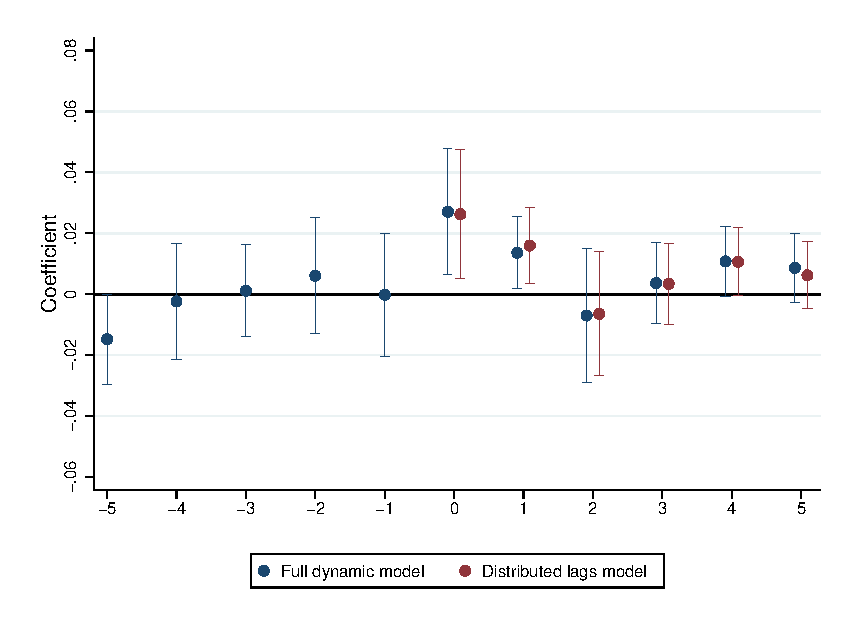
\includegraphics[width = \textwidth]
    	{../../analysis/first_differences/output/fd_models_coeffs_w5.eps}
    \end{subfigure}
    \begin{subfigure}[b]{0.8\textwidth}
    	\caption{Cumulative sum}
    	\label{fig:dynamic_model_cumsum}
    	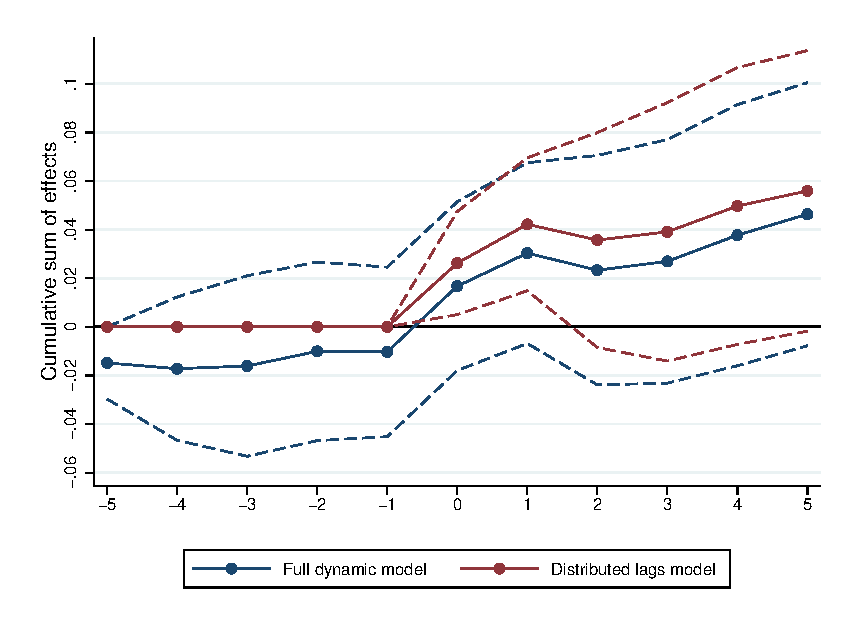
\includegraphics[width = \textwidth]
    	{../../analysis/first_differences/output/fd_models_cumsum.eps}
    \end{subfigure}
    \begin{minipage}{0.95\textwidth} \footnotesize
		\vspace{2mm} 
		\textit{Notes}: Panel (a) shows the estimated coefficients for the \textit{dynamic} model from 
		 \autoref{eq:leads_lags}, together with a lags only model. Panel (b) shows the cumulative 
		 effect of the coefficients reported in panel (a) for the two model specifications. Estimates
		 for the full dynamic model are reported in \autoref{tab:dynamic_lags_leads_main}. In both panels, 
		 90 percent confidence intervals are reported. 
	\end{minipage}
\end{figure}

To directly account for the presence of zipcode level rent dynamics, we further test our results by 
estimating a \textit{dynamic} DiD model that controls for the lagged value of the changes in rents 
(\autoref{eq:ab_panel}). We compare that with our baseline estimates in 
\autoref{tab:horse_race_ab}: columns 1, 2, and 3 show coefficients from equations \eqref{eq:did}, 
\eqref{eq:leads_lags}, and a lags only model respectively. In columns 4 and 5, we allow for full blown 
dynamics in the dependent variable and we recover the coefficients using instrumental variables 
following the classic \textcite{ArellanoBond1991} approach --using deeper lags of the dependent 
variable to instrument for the lagged dependent variable-- for the cases with and without leads. 
In columns 6 and 7 we show estimates from the model in equation \ref{eq:ab_panel} but instrumenting 
the lagged dependent variable with the sixth MW change lag as in \textcite{MeerWest2016}. Our 
effects are robust to all of this stringent tests: the same-month change in rents following a 10 
percent increase in MW is consistently estimated between 0.25 and 0.3 percent. 


\subsection{External Validity and Data Sensitivity}\label{sec:sample_rest}

Our results suggest a noticeable impact of MW policies on the rental housing market. However, as 
explained in \autoref{sec:data}, the number of zipcodes included in the final sample is only a 
small portion of the total U.S., and they come from more urban and richer neighborhoods that likely 
have a dynamic housing market. This limited sample size might hinder the external validity of the 
estimated effect. Additionally, the zipcodes included in the final sample are the ones appearing 
earlier in the Zillow data (i.e. zipcodes whose rent data are available since January 2010), and 
this might result in unobserved differences affecting sample selection.

We test the sensitivity with respect to our sample restrictions in two ways. First, we extend our 
panel by including the full set of zipcodes for which there is available rent data. This, on one 
hand, doubles the sample size (we now use the full $3,316$ zipcode in the Zillow rent data for 
single family, condos and cooperative houses), but, on the other hand, makes the composition of 
zipcodes vary over time by including, as they enter the sample, zipcodes whose time series start 
later than January 2010. Therefore, to fully exploit our data we estimate models using an unbalanced 
panel but controlling for ``cohort $\times$ period" fixed effects. We do this both for the \textit{static}, 
the \textit{dynamic} model. In this way, 
we are able to compare treated and untreated zipcodes with the same panel length.

Secondly, we assess the representativeness of our estimates by re-weighting zipcodes so as to match 
socio-demographic characteristics of the zipcodes in the top-100 CBSA. We do this by applying the 
entropy balancing procedure developed by \cite{hainmueller2012entropy} on the following zipcode 
level demographics: share of rental houses, share of African-American residents, share of college 
graduates, and median income. We target averages from \autoref{tab:desc_stats}, column 
2.\footnote{The entropy balancing procedure consists of a re-weighting scheme that assigns a scalar 
	weight to every unit such that the re-weighted sample matches moments of a target population. We 
	implement this by leveraging the \texttt{STATA} package \texttt{ebalance} described in 
	\textcite{hainmueller2013ebalance}.} We subsequently re-estimate our models with weighted regressions.


%In 
%\autoref{tab:comparison_unbal_base} we show that that the estimated effects for the different models 
%remain widely unchanged. In \autoref{fig:dynamic_dd_comparison}, panel (a) we compare 
%\textit{dynamic} DiD estimates obtained using the baseline sample and the unbalanced sample. Using 
%the unbalanced panel, our estimates are slightly lower but they are largely identical to the baseline 
%results.
%
%
%The results shown in \autoref{fig:dynamic_dd_comparison}, panel(b) confirm what we found in our 
%baseline case, although point estimates are somewhat higher. Note that the simultaneous effect from 
%the \textit{dynamic} DiD model presents the only statistically significant post-treatment 
%coefficient. The effect in month $t+1$ becomes indeed smaller and not significant, suggesting how 
%the baseline model might overestimate the persistence of the true average effect. A comparison with 
%the \textit{static} DiD estimate supports this finding: $\hat{\beta}$ from \autoref{eq:did} and 
%$\hat{\beta}_{t}$ from \autoref{eq:leads_lags} are almost identical, identifying an elasticity on 
%rents of approximately $0.036$ (\autoref{tab:comparison_wgt_base}).

%\begin{figure}[htb!]
%    \caption{Comparison between dynamic DiD models}
%    \label{fig:dynamic_dd_comparison}
%    \centering
%    \begin{subfigure}[b]{0.8\textwidth}
%        \caption{Unbalanced panel}
%        \includegraphics[width = \textwidth]
%        {../../analysis/first_differences_unbal/output/fd_model_comparison_unbal.png}
%    \end{subfigure}
%    \begin{subfigure}[b]{0.8\textwidth}
%        \caption{Reweighted panel}
%        \includegraphics[width = \textwidth]
%        {../../analysis/first_differences_wgt/output/fd_model_comparison_wgt.png}
%    \end{subfigure}
%    \begin{minipage}{0.95\textwidth} \footnotesize
%		\vspace{2mm} 
%		\textit{Notes}: The plot compares results obtained from the baseline panel summarized in 
%		\autoref{tab:desc_stats}, column 4 with those obtained from the full unbalanced panel (a), 
%		and with the reweighted baseline panel (b). Each subfigure compares estimated coefficients 
%		for the \textit{dynamic DiD} models calculated through \autoref{eq:leads_lags}, and point 
%		estimates for the cumulative effect of MW on rents estimated through \autoref{eq:lags}.   
%	\end{minipage}
%\end{figure}

\begin{table}[h!]\centering
	\caption{External Validity and Sensitivity Robustness Checks}
	\label{tab:wgt_unbal_comparison}
	\resizebox{0.8\textwidth}{!}{
		{
\def\sym#1{\ifmmode^{#1}\else\(^{#1}\)\fi}
\begin{tabular}{l*{4}{c}}
\hline\hline
          &\multicolumn{1}{c}{(1)}&\multicolumn{1}{c}{(2)}&\multicolumn{1}{c}{(3)}&\multicolumn{1}{c}{(4)}\\
          &\multicolumn{1}{c}{Baseline}&\multicolumn{1}{c}{Unbalanced}&\multicolumn{1}{c}{\shortstack{Unbalanced \\ + reweighted}}&\multicolumn{1}{c}{Reweighted}\\
\hline
Static Effect&   0.0257\sym{**} &   0.0225\sym{*}  &   0.0229         &   0.0389\sym{***}\\
          & (0.0124)         & (0.0115)         & (0.0139)         & (0.0131)         \\
\hline
\vspace{-2mm}&                  &                  &                  &                  \\
Cumulative effect&0.0595\sym{*}         &0.0534\sym{*}         &   0.0503         &0.0737\sym{*}         \\
          & (0.0343)         & (0.0297)         & (0.0358)         & (0.0428)         \\
\hline    &                  &                  &                  &                  \\
Wage controls&      Yes         &      Yes         &      Yes         &      Yes         \\
Employment controls&      Yes         &      Yes         &      Yes         &      Yes         \\
Establishment-count controls&      Yes         &      Yes         &      Yes         &      Yes         \\
R-squared &    0.022         &    0.053         &    0.055         &    0.023         \\
Observations&  107,781         &  182,608         &  182,577         &  107,781         \\
\hline\hline
\end{tabular}
}

	}
	\begin{minipage}{\textwidth}\footnotesize
	\vspace{3mm}	
	\textit{Notes:} The table shows the static and cumulative effects caused by a $1$ percent
	change in MW on rents. The static effect is estimated by $\hat{\beta}$ from \autoref{eq:did};
	the cumulative effect is obtained as a linear combination of the $\beta_{t+r}$ coefficients from 
	a distributed-lags model based on \autoref{eq:leads_lags}: 
	$\sum\limits_{r = 0}^5 \hat{\beta}_{t+r}$. All specifications include time fixed effects, 
	and additionally use QCEW data to control for wages, employment and number of establishments 
	for the ``Professional and business services", ``Information", and ``Financial activities" industries.
	Standard errors clustered at the state level are
	reported in parenthesis. \\
	Significance codes: *** $p < 0.01$, ** $p < 0.05$, * $p < 0.1$. 	
	\end{minipage}
\end{table}

In \autoref{tab:wgt_unbal_comparison} we compare baseline results with those obtained from the 
two exercises. For each specification, we show the estimated impact
from the \textit{static} model and the cumulative effect obtained from the distributed lag model. Column 
2 highlights how expanding the underlying sample size mildly lowers the impact of MW on rents, but 
it does not change the overall pattern. Notably, the estimates' precision increases in particular for 
the cumulative effect (we clearly see this in \autoref{fig:dynamic_wgt_unabl_comp}, panel a, where 
the standard error obtained for $\hat{\beta}_{t+2}$  becomes now comparable to 
that of the other estimated coefficients). A 10 percent increase in the MW leads to an simultaneous 
$0.23$ percent increase in rents, growing to $0.53$ percent in a 6-months span. Column 3 shows 
the results obtained from estimating weighted models. Although the overall dynamic remains unchanged, 
the effect of a 10 percent increase in MW now causes a $0.39$ percent increase in the same month, and 
a $0.73$ percent after 6 months. %ADD INTERPRETATION?



%%%%%%%%%%%%%%%%%%%%%%%%%%%%%%%%%%%%%%%%%%%%%%%%%%%%%%%%%%%%%%%%%%%%%%%%%%%%%%%%%
\subsection{The Heterogeneity of MW Impacts on Rents}\label{sec:heter}

Our baseline results in \autoref{sec:baseline_results} have documented the presence of a causal 
impact of MW on rents, and the effect appears robust to multiple checks introduced in Sections 
\ref{sec:sample_rest}. We now investigate the heterogeneity of such effect 
by characterizing zipcodes based on socio-demographic characteristics. The goal of this exercise is 
to understand who are the ``winners" and ``losers" when rents increase 
due to new MW provisions. We look at zipcode characteristics to identify which sub-population ends 
up paying more in rents.

\autoref{tab:fd_model_het} shows the estimated coefficients for the interaction between changes in 
(log) MW and quartiles of the distribution for several demographics. Column 1 shows how 
the effect does not appear to disproportionately impact zipcodes in the lower quartiles of the 
median income distribution: none of the interaction coefficients is statistically significant. A possible 
explanation is that zipcode median income might still be associated with
substantial variation in the relative share of MW residents directly affected by the income shock.
[]ADD  REFERENCE TO MW BITE, SEE AUTOR ET AL 2016]. 
In column 2 we focus on the zipcode-level unemployment rate. Not surprisingly, we find that the 
strongest effect is localized in the $4^{th}$ quartile of the distribution, 0.043 (s.e. 0.017). 
Estimates lose significance in the remaining part of the distribution: similarly to column 1, we 
find not-significant not-monotone estimates in the middle quartiles, while the effect is a clear 
zero in the bottom quarter. Perhaps not surprisingly, classifying zipcodes according to a demographic
characteristic more closely associated with the status of MW earner indeed suggest how the bulk of the 
impact is concentrated in areas where is more likely to have MW residents. Column 3 
focuses on the share of college graduates. In a similar fashion, the estimates 
confirm that lower educated neighborhoods experience a larger rent increase: there is a 
clear divide between above median zipcodes showing zero and not significant effects, and below 
median ones where a 10 percent increase in MW leads to a 0.45 and a 0.36 percent rent increase for 
the $2^{nd}$ and $1^{st}$ quartiles, respectively. In column 4 we show the impact across 
the distribution over share of African-American residents. The effect of MW changes 
on rents is neither significant in the $1^{st}$ quarter ($0.017$, s.e. $0.016$), nor in the 
$2^{nd}$ and $3^{rd}$ (although we have a higher point estimate). In the $4^{th}$ however, effect 
becomes statistically significant with a 10 percent increase in MW leading to a $0.4$ percent rent 
increase. Lastly, in column (5) we reports the estimated interaction coefficients obtained with quartiles 
based on the share of residents between 15 and 24 years old, a strong predictor of MW worker status 
(ADD REFERENCE). The largest impact is recorded in zipcodes in the $4^{th}$ quartile ($0.041$, s.e. $0.01$), 
while it becomes smaller and not significant in the remaining quartiles.  Overall, rent increases appear to be localized 
in those neighborhoods characterized by demographics historically associated with the profile of MW workers, 
thus suggesting how the very groups originally targeted by MW provisions may be those experiencing higher 
rent extraction. 

\begin{table}[h!]
    \caption{Heterogeneity Results - static DiD model}
    \label{tab:fd_model_het}
    \centering
    \resizebox{0.95\textwidth}{!}{             
	    \vspace{0pt}    
	    {
\def\sym#1{\ifmmode^{#1}\else\(^{#1}\)\fi}
\begin{tabular}{l*{4}{c}}
\hline\hline
          &\multicolumn{1}{c}{(1)}&\multicolumn{1}{c}{(2)}&\multicolumn{1}{c}{(3)}&\multicolumn{1}{c}{(4)}\\
          &\multicolumn{1}{c}{Median Income}&\multicolumn{1}{c}{Rental House (\%)}&\multicolumn{1}{c}{College Grad. (\%)}&\multicolumn{1}{c}{African Am. (\%)}\\
\hline
$\Delta \ln(MW) \times 1^{st} qtl$&   0.0395\sym{*}  &   0.0317\sym{*}  &   0.0373\sym{*}  &   0.0178         \\
          & (0.0223)         & (0.0169)         & (0.0196)         & (0.0163)         \\
[1em]
$\Delta \ln(MW) \times 2^{nd} qtl$&   0.0202         &   0.0123         &   0.0473\sym{**} &   0.0218         \\
          & (0.0144)         & (0.0179)         & (0.0222)         & (0.0163)         \\
[1em]
$\Delta \ln(MW) \times 3^{rd} qtl$&   0.0304         &   0.0140         &   0.0258         &   0.0231\sym{*}  \\
          & (0.0252)         & (0.0227)         & (0.0214)         & (0.0133)         \\
[1em]
$\Delta \ln(MW) \times 4^{th} qtl$&   0.0133         &   0.0427\sym{***}&-0.000369         &   0.0419\sym{**} \\
          & (0.0130)         & (0.0156)         & (0.0116)         & (0.0164)         \\
\hline
R-squared &    0.024         &    0.024         &    0.024         &    0.024         \\
Observations&  112,232         &  112,232         &  112,232         &  112,232         \\
\hline\hline
\end{tabular}
}

    }
    \begin{minipage}{0.95\textwidth} \footnotesize
		\vspace{3mm}
		\textit{Notes}: The table reports estimates for $\beta_{q}$, $q=\{1, 2, 3, 4\}$ from 
		\autoref{eq:diff_main_hetero} when differentiating zipcodes based on several 
		socio-demographics from the 2010 Census and the 5-year 2008-2012 ACS. All specifications 
		include time fixed effects, and additionally use QCEW data to control for wages, 
		employment and number of establishments for the ``Professional and business 
		services", ``Information", and ``Financial activities" industries.
		Standard errors clustered at the state level are
		reported in parenthesis. \\
		Standard errors clustered at the state level. *** $p < 0.01$, ** $p < 0.05$, * $p < 0.1$.  
	\end{minipage}
\end{table}
